\documentclass[10pt,a4paper]{article}
\usepackage[utf8]{inputenc}
\usepackage[english,german]{babel}
\usepackage{utopia}
\usepackage[left=1cm,top=2cm,right=1cm,bottom=2cm]{geometry}
\usepackage[parfill]{parskip}
\usepackage{makeidx}
\usepackage[onehalfspacing]{setspace}
\usepackage{fancyhdr}
\usepackage{lastpage}
\usepackage{hyperref}
\usepackage{multicol}
\usepackage{graphicx}
\renewcommand{\sffamily}{phv}

\newcommand{\titleText}{Spick Mathematik\\Stereometrie}
\newcommand{\authorText}{Patrick Günthard\\6MT13v}
\newcommand{\dateText}{\today}

\title{\titleText}
\author{\authorText}
\date{\dateText}

\pagestyle{fancy}
\fancyhf{}

\lhead{\titleText}
\rhead{\authorText}
\cfoot{\thepage \space von \pageref{LastPage}}

\begin{document}
	\begin{multicols}{4}
		
		\section{Kreisyzlinder}
		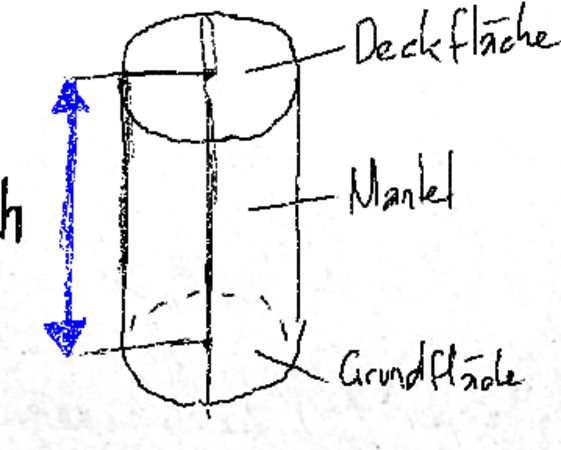
\includegraphics[width=3cm]{imgs/zyl1}
		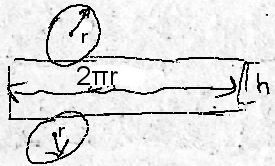
\includegraphics[width=3cm]{imgs/zyl2}
		
		
		\textbf{Mantelfläche:}\\
		\(M = h * 2\pi r\)\\
		\textbf{Grundfläche}\\
		\(G = \pi r^2 \)\\
		\textbf{Gesamte Fläche:}\\
		\(S=M + 2G\)\\
		\textbf{Volumen:}\\
		\(V = G * h \)\\
		
		\section{Kreiskegel}
		
		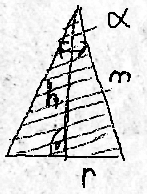
\includegraphics[width=3cm]{imgs/keg1}
		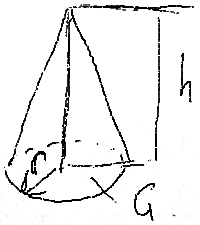
\includegraphics[width=3cm]{imgs/keg2}
		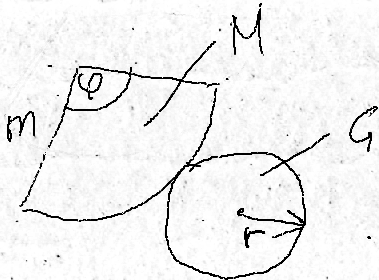
\includegraphics[width=3cm]{imgs/keg3}
		
		\textbf{Mantelfläche:}\\
		\(M = \pi rm \)\\
		\textbf{Gesamtfläche:}\\
		\(S = \pi r (r + m) \)\\
		\textbf{Volumen:}\\
		\(V=\frac{1}{3} G h = \frac{\pi}{3}r^2 h\)\\
		\textbf{Relationen}\\
		\( \widehat{\phi} = \frac{2\pi r}{m} \)
		
		\section{Kegelstumpf}
		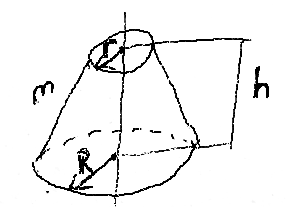
\includegraphics[width=3cm]{imgs/kegs1}\\
		\textbf{Der gerade Kegelstumpf}\\
		\(V = \frac{\pi}{3}h (r^2 + R^2 + Rr) \)\\
		\textbf{Mantelfläche}\\
		\(M = \pi m (r + R) \)
		
		\section{Kugel}
		\subsection{Ganze Kugel}
		\( V = \frac{4\pi}{3}r^3 \)\\
		\( S = 4\pi r^2 \)
		
		\subsection{Kugelsektor}
		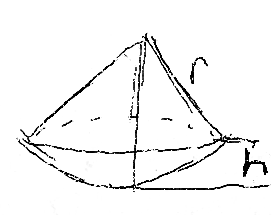
\includegraphics[width=3cm]{imgs/kugsek}\\
		\(V = \frac{2\pi}{3} r^2 h \)
		
		\subsection{Kugelsegment}
		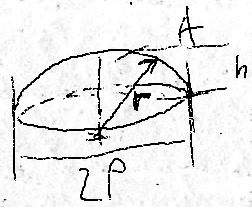
\includegraphics[width=3cm]{imgs/kugseg}\\
		\( V = \frac{\pi}{3} h^2 (3r - h) \)\\
		\( V = \frac{pi}{6} h (3 \rho^2 + h^2) \)\\
		\( S = A + \pi \rho^2 \)\\
		\( A = 2 \pi r h \)
		
		\subsection{Kugelschicht}
		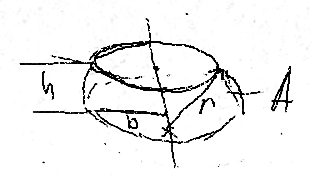
\includegraphics[width=3cm]{imgs/kugsch}\\
		\( V = \frac{\pi}{6} h (3a^2 + b^2 + h^2) \)\\
		\( S = A + \pi (a^2 + b^2) \)\\
		\( A = 2 \pi r h \)
	
		\section{Guldnische Regeln}
		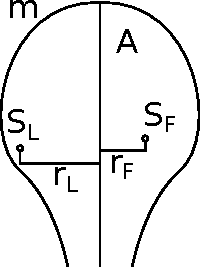
\includegraphics[width=3cm]{imgs/rotat}\\
		\( V = 2 \pi r_F A \)\\
		\( M = 2 \pi r_L m \)\\
		\textbf{Flächenschwerpunkt Dreieck}\\
		\( x_S = \frac{x_1 + x_2 + x_3}{3} \)\\
		\( y_S = \frac{y_1 + y_2 + y_3}{3} \)
		
		\section{Ähnliche Körper}
		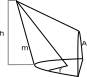
\includegraphics[width=3cm]{imgs/similar}\\
		\( k = \frac{h'}{h} = \frac{r'}{r} = \frac{m'}{m} \)\\
		\( k^2 = \frac{G'}{G} = \frac{M'}{M} = \frac{A'}{A} = \frac{S'}{S} \)\\
		\( V = \frac{V'}{V} \)
	\end{multicols}
\end{document}